\documentclass[twoside]{book}

% Packages required by doxygen
\usepackage{fixltx2e}
\usepackage{calc}
\usepackage{doxygen}
\usepackage[export]{adjustbox} % also loads graphicx
\usepackage{graphicx}
\usepackage[utf8]{inputenc}
\usepackage{makeidx}
\usepackage{multicol}
\usepackage{multirow}
\PassOptionsToPackage{warn}{textcomp}
\usepackage{textcomp}
\usepackage[nointegrals]{wasysym}
\usepackage[table]{xcolor}

% Font selection
\usepackage[T1]{fontenc}
\usepackage[scaled=.90]{helvet}
\usepackage{courier}
\usepackage{amssymb}
\usepackage{sectsty}
\renewcommand{\familydefault}{\sfdefault}
\allsectionsfont{%
  \fontseries{bc}\selectfont%
  \color{darkgray}%
}
\renewcommand{\DoxyLabelFont}{%
  \fontseries{bc}\selectfont%
  \color{darkgray}%
}
\newcommand{\+}{\discretionary{\mbox{\scriptsize$\hookleftarrow$}}{}{}}

% Page & text layout
\usepackage{geometry}
\geometry{%
  a4paper,%
  top=2.5cm,%
  bottom=2.5cm,%
  left=2.5cm,%
  right=2.5cm%
}
\tolerance=750
\hfuzz=15pt
\hbadness=750
\setlength{\emergencystretch}{15pt}
\setlength{\parindent}{0cm}
\setlength{\parskip}{3ex plus 2ex minus 2ex}
\makeatletter
\renewcommand{\paragraph}{%
  \@startsection{paragraph}{4}{0ex}{-1.0ex}{1.0ex}{%
    \normalfont\normalsize\bfseries\SS@parafont%
  }%
}
\renewcommand{\subparagraph}{%
  \@startsection{subparagraph}{5}{0ex}{-1.0ex}{1.0ex}{%
    \normalfont\normalsize\bfseries\SS@subparafont%
  }%
}
\makeatother

% Headers & footers
\usepackage{fancyhdr}
\pagestyle{fancyplain}
\fancyhead[LE]{\fancyplain{}{\bfseries\thepage}}
\fancyhead[CE]{\fancyplain{}{}}
\fancyhead[RE]{\fancyplain{}{\bfseries\leftmark}}
\fancyhead[LO]{\fancyplain{}{\bfseries\rightmark}}
\fancyhead[CO]{\fancyplain{}{}}
\fancyhead[RO]{\fancyplain{}{\bfseries\thepage}}
\fancyfoot[LE]{\fancyplain{}{}}
\fancyfoot[CE]{\fancyplain{}{}}
\fancyfoot[RE]{\fancyplain{}{\bfseries\scriptsize Generated by Doxygen }}
\fancyfoot[LO]{\fancyplain{}{\bfseries\scriptsize Generated by Doxygen }}
\fancyfoot[CO]{\fancyplain{}{}}
\fancyfoot[RO]{\fancyplain{}{}}
\renewcommand{\footrulewidth}{0.4pt}
\renewcommand{\chaptermark}[1]{%
  \markboth{#1}{}%
}
\renewcommand{\sectionmark}[1]{%
  \markright{\thesection\ #1}%
}

% Indices & bibliography
\usepackage{natbib}
\usepackage[titles]{tocloft}
\setcounter{tocdepth}{3}
\setcounter{secnumdepth}{5}
\makeindex

% Hyperlinks (required, but should be loaded last)
\usepackage{ifpdf}
\ifpdf
  \usepackage[pdftex,pagebackref=true]{hyperref}
\else
  \usepackage[ps2pdf,pagebackref=true]{hyperref}
\fi
\hypersetup{%
  colorlinks=true,%
  linkcolor=blue,%
  citecolor=blue,%
  unicode%
}

% Custom commands
\newcommand{\clearemptydoublepage}{%
  \newpage{\pagestyle{empty}\cleardoublepage}%
}

\usepackage{caption}
\captionsetup{labelsep=space,justification=centering,font={bf},singlelinecheck=off,skip=4pt,position=top}

%===== C O N T E N T S =====

\begin{document}

% Titlepage & ToC
\hypersetup{pageanchor=false,
             bookmarksnumbered=true,
             pdfencoding=unicode
            }
\pagenumbering{alph}
\begin{titlepage}
\vspace*{7cm}
\begin{center}%
{\Large P\+I\+D-\/\+Controller }\\
\vspace*{1cm}
{\large Generated by Doxygen 1.8.13}\\
\end{center}
\end{titlepage}
\clearemptydoublepage
\pagenumbering{roman}
\tableofcontents
\clearemptydoublepage
\pagenumbering{arabic}
\hypersetup{pageanchor=true}

%--- Begin generated contents ---
\chapter{Class Index}
\section{Class List}
Here are the classes, structs, unions and interfaces with brief descriptions\+:\begin{DoxyCompactList}
\item\contentsline{section}{\hyperlink{classPID}{P\+ID} }{\pageref{classPID}}{}
\end{DoxyCompactList}

\chapter{File Index}
\section{File List}
Here is a list of all documented files with brief descriptions\+:\begin{DoxyCompactList}
\item\contentsline{section}{include/\hyperlink{pid_8hpp}{pid.\+hpp} \\*Header file for \hyperlink{classPID}{P\+ID} Controller }{\pageref{pid_8hpp}}{}
\item\contentsline{section}{test/\hyperlink{main_8cpp}{main.\+cpp} \\*Main file for test cases }{\pageref{main_8cpp}}{}
\item\contentsline{section}{test/\hyperlink{test_8cpp}{test.\+cpp} \\*Test file for \hyperlink{classPID}{P\+ID} Controller }{\pageref{test_8cpp}}{}
\end{DoxyCompactList}

\chapter{Class Documentation}
\hypertarget{classPID}{}\section{P\+ID Class Reference}
\label{classPID}\index{P\+ID@{P\+ID}}
\subsection*{Public Member Functions}
\begin{DoxyCompactItemize}
\item 
\hyperlink{classPID_a74e83c18b71000d5e9d9ff4f0832045c}{P\+ID} (double Kp, double Ki, double Kd, double dt, double min, double max)
\begin{DoxyCompactList}\small\item\em Construct a new \hyperlink{classPID}{P\+ID} object. \end{DoxyCompactList}\item 
double \hyperlink{classPID_ac3e8ba5eef028a4c61af628bbd351734}{calculate\+Error\+Integral} (double error)
\begin{DoxyCompactList}\small\item\em Calculates the error integral. \end{DoxyCompactList}\item 
double \hyperlink{classPID_a58446fa1dd31e998351133adbfe0d37c}{calculate\+Error\+Derivative} (double error)
\begin{DoxyCompactList}\small\item\em Calculates the error derivative. \end{DoxyCompactList}\item 
double \hyperlink{classPID_a5ea88b2d321c2c1f24aded4bd660c7c4}{compute\+Output} (double initial\+\_\+state, double final\+\_\+state)
\begin{DoxyCompactList}\small\item\em calculates the velocity output \end{DoxyCompactList}\item 
double \hyperlink{classPID_a52625de61b1b2977b2c26ddb2698f14e}{get\+Kp} ()
\begin{DoxyCompactList}\small\item\em Get the Kp parameter. \end{DoxyCompactList}\item 
double \hyperlink{classPID_a39997546e8d1025c6c867e31e8b8e916}{get\+Kd} ()
\begin{DoxyCompactList}\small\item\em Get the Kd parameter. \end{DoxyCompactList}\item 
double \hyperlink{classPID_a89dedae29ef5a1359fd438824523bfc5}{get\+Ki} ()
\begin{DoxyCompactList}\small\item\em Get the Ki parameter. \end{DoxyCompactList}\item 
\mbox{\Hypertarget{classPID_a13ac471272cc1b8da59b77de83abb46d}\label{classPID_a13ac471272cc1b8da59b77de83abb46d}} 
void \hyperlink{classPID_a13ac471272cc1b8da59b77de83abb46d}{check\+Parameters} ()
\begin{DoxyCompactList}\small\item\em check parameters \end{DoxyCompactList}\end{DoxyCompactItemize}


\subsection{Constructor \& Destructor Documentation}
\mbox{\Hypertarget{classPID_a74e83c18b71000d5e9d9ff4f0832045c}\label{classPID_a74e83c18b71000d5e9d9ff4f0832045c}} 
\index{P\+ID@{P\+ID}!P\+ID@{P\+ID}}
\index{P\+ID@{P\+ID}!P\+ID@{P\+ID}}
\subsubsection{\texorpdfstring{P\+I\+D()}{PID()}}
{\footnotesize\ttfamily P\+I\+D\+::\+P\+ID (\begin{DoxyParamCaption}\item[{double}]{Kp,  }\item[{double}]{Ki,  }\item[{double}]{Kd,  }\item[{double}]{dt,  }\item[{double}]{min,  }\item[{double}]{max }\end{DoxyParamCaption})}



Construct a new \hyperlink{classPID}{P\+ID} object. 


\begin{DoxyParams}{Parameters}
{\em Kp} & (double) -\/ Proportional constant \\
\hline
{\em Ki} & (double) -\/ Integral constant \\
\hline
{\em Kd} & (double) -\/ Derivative constant \\
\hline
{\em dt} & (double) -\/ time \\
\hline
{\em previous\+\_\+error} & (double) previous error \\
\hline
{\em integral\+\_\+sum} & (double) the integration summation \\
\hline
\end{DoxyParams}


\subsection{Member Function Documentation}
\mbox{\Hypertarget{classPID_a58446fa1dd31e998351133adbfe0d37c}\label{classPID_a58446fa1dd31e998351133adbfe0d37c}} 
\index{P\+ID@{P\+ID}!calculate\+Error\+Derivative@{calculate\+Error\+Derivative}}
\index{calculate\+Error\+Derivative@{calculate\+Error\+Derivative}!P\+ID@{P\+ID}}
\subsubsection{\texorpdfstring{calculate\+Error\+Derivative()}{calculateErrorDerivative()}}
{\footnotesize\ttfamily double P\+I\+D\+::calculate\+Error\+Derivative (\begin{DoxyParamCaption}\item[{double}]{error }\end{DoxyParamCaption})}



Calculates the error derivative. 


\begin{DoxyParams}{Parameters}
{\em initial\+\_\+state} & (double) -\/ initial state \\
\hline
{\em final\+\_\+state} & (double) -\/ final state \\
\hline
\end{DoxyParams}
\begin{DoxyReturn}{Returns}
double (double) -\/ error derivative 
\end{DoxyReturn}
\mbox{\Hypertarget{classPID_ac3e8ba5eef028a4c61af628bbd351734}\label{classPID_ac3e8ba5eef028a4c61af628bbd351734}} 
\index{P\+ID@{P\+ID}!calculate\+Error\+Integral@{calculate\+Error\+Integral}}
\index{calculate\+Error\+Integral@{calculate\+Error\+Integral}!P\+ID@{P\+ID}}
\subsubsection{\texorpdfstring{calculate\+Error\+Integral()}{calculateErrorIntegral()}}
{\footnotesize\ttfamily double P\+I\+D\+::calculate\+Error\+Integral (\begin{DoxyParamCaption}\item[{double}]{error }\end{DoxyParamCaption})}



Calculates the error integral. 


\begin{DoxyParams}{Parameters}
{\em initial\+\_\+state} & (double) -\/ initial state \\
\hline
{\em final\+\_\+state} & (double) -\/ final state \\
\hline
\end{DoxyParams}
\begin{DoxyReturn}{Returns}
(double) -\/ error integral 
\end{DoxyReturn}
\mbox{\Hypertarget{classPID_a5ea88b2d321c2c1f24aded4bd660c7c4}\label{classPID_a5ea88b2d321c2c1f24aded4bd660c7c4}} 
\index{P\+ID@{P\+ID}!compute\+Output@{compute\+Output}}
\index{compute\+Output@{compute\+Output}!P\+ID@{P\+ID}}
\subsubsection{\texorpdfstring{compute\+Output()}{computeOutput()}}
{\footnotesize\ttfamily double P\+I\+D\+::compute\+Output (\begin{DoxyParamCaption}\item[{double}]{initial\+\_\+state,  }\item[{double}]{final\+\_\+state }\end{DoxyParamCaption})}



calculates the velocity output 


\begin{DoxyParams}{Parameters}
{\em initial\+\_\+state} & (double) -\/ initial state \\
\hline
{\em final\+\_\+state} & (double) -\/ final state \\
\hline
\end{DoxyParams}
\begin{DoxyReturn}{Returns}
(double) -\/ final velocity 
\end{DoxyReturn}
\mbox{\Hypertarget{classPID_a39997546e8d1025c6c867e31e8b8e916}\label{classPID_a39997546e8d1025c6c867e31e8b8e916}} 
\index{P\+ID@{P\+ID}!get\+Kd@{get\+Kd}}
\index{get\+Kd@{get\+Kd}!P\+ID@{P\+ID}}
\subsubsection{\texorpdfstring{get\+Kd()}{getKd()}}
{\footnotesize\ttfamily double P\+I\+D\+::get\+Kd (\begin{DoxyParamCaption}{ }\end{DoxyParamCaption})}



Get the Kd parameter. 

\begin{DoxyReturn}{Returns}
double 
\end{DoxyReturn}
\mbox{\Hypertarget{classPID_a89dedae29ef5a1359fd438824523bfc5}\label{classPID_a89dedae29ef5a1359fd438824523bfc5}} 
\index{P\+ID@{P\+ID}!get\+Ki@{get\+Ki}}
\index{get\+Ki@{get\+Ki}!P\+ID@{P\+ID}}
\subsubsection{\texorpdfstring{get\+Ki()}{getKi()}}
{\footnotesize\ttfamily double P\+I\+D\+::get\+Ki (\begin{DoxyParamCaption}{ }\end{DoxyParamCaption})}



Get the Ki parameter. 

\begin{DoxyReturn}{Returns}
double 
\end{DoxyReturn}
\mbox{\Hypertarget{classPID_a52625de61b1b2977b2c26ddb2698f14e}\label{classPID_a52625de61b1b2977b2c26ddb2698f14e}} 
\index{P\+ID@{P\+ID}!get\+Kp@{get\+Kp}}
\index{get\+Kp@{get\+Kp}!P\+ID@{P\+ID}}
\subsubsection{\texorpdfstring{get\+Kp()}{getKp()}}
{\footnotesize\ttfamily double P\+I\+D\+::get\+Kp (\begin{DoxyParamCaption}{ }\end{DoxyParamCaption})}



Get the Kp parameter. 

\begin{DoxyReturn}{Returns}
double 
\end{DoxyReturn}


The documentation for this class was generated from the following file\+:\begin{DoxyCompactItemize}
\item 
include/\hyperlink{pid_8hpp}{pid.\+hpp}\end{DoxyCompactItemize}

\chapter{File Documentation}
\hypertarget{pid_8hpp}{}\section{include/pid.hpp File Reference}
\label{pid_8hpp}\index{include/pid.\+hpp@{include/pid.\+hpp}}


Header file for \hyperlink{classPID}{P\+ID} Controller.  


{\ttfamily \#include $<$iostream$>$}\newline
{\ttfamily \#include $<$stdexcept$>$}\newline
Include dependency graph for pid.\+hpp\+:\nopagebreak
\begin{figure}[H]
\begin{center}
\leavevmode
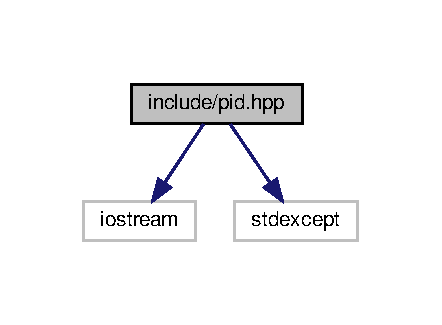
\includegraphics[width=212pt]{pid_8hpp__incl}
\end{center}
\end{figure}
This graph shows which files directly or indirectly include this file\+:\nopagebreak
\begin{figure}[H]
\begin{center}
\leavevmode
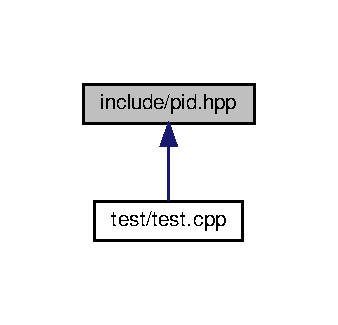
\includegraphics[width=162pt]{pid_8hpp__dep__incl}
\end{center}
\end{figure}
\subsection*{Classes}
\begin{DoxyCompactItemize}
\item 
class \hyperlink{classPID}{P\+ID}
\end{DoxyCompactItemize}


\subsection{Detailed Description}
Header file for \hyperlink{classPID}{P\+ID} Controller. 

\begin{DoxyAuthor}{Author}
Siddharth Telang (\href{mailto:stelang@umd.edu}{\tt stelang@umd.\+edu}) 

Dani Lerner (\href{mailto:dalerner@umd.edu}{\tt dalerner@umd.\+edu}) 
\end{DoxyAuthor}
\begin{DoxyVersion}{Version}
0.\+1 
\end{DoxyVersion}
\begin{DoxyDate}{Date}
2021-\/09-\/30
\end{DoxyDate}
Copyright (c) 2021 Pair A 
\hypertarget{main_8cpp}{}\section{test/main.cpp File Reference}
\label{main_8cpp}\index{test/main.\+cpp@{test/main.\+cpp}}


main file for test cases  


{\ttfamily \#include $<$gtest/gtest.\+h$>$}\newline
Include dependency graph for main.\+cpp\+:\nopagebreak
\begin{figure}[H]
\begin{center}
\leavevmode
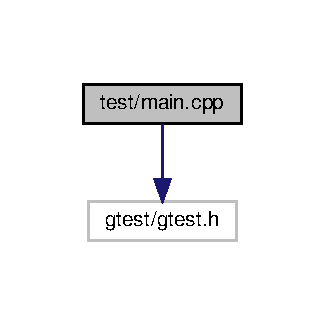
\includegraphics[width=156pt]{main_8cpp__incl}
\end{center}
\end{figure}
\subsection*{Functions}
\begin{DoxyCompactItemize}
\item 
\mbox{\Hypertarget{main_8cpp_a3c04138a5bfe5d72780bb7e82a18e627}\label{main_8cpp_a3c04138a5bfe5d72780bb7e82a18e627}} 
int {\bfseries main} (int argc, char $\ast$$\ast$argv)
\end{DoxyCompactItemize}


\subsection{Detailed Description}
main file for test cases 

\begin{DoxyAuthor}{Author}
Siddharth Telang (\href{mailto:stelang@umd.edu}{\tt stelang@umd.\+edu}) 

Dani Lerner (\href{mailto:dalerner@umd.edu}{\tt dalerner@umd.\+edu}) 
\end{DoxyAuthor}
\begin{DoxyVersion}{Version}
0.\+1 
\end{DoxyVersion}
\begin{DoxyDate}{Date}
2021-\/09-\/30
\end{DoxyDate}
Copyright (c) 2021 Pair A 
\hypertarget{test_8cpp}{}\section{test/test.cpp File Reference}
\label{test_8cpp}\index{test/test.\+cpp@{test/test.\+cpp}}


Test file for \hyperlink{classPID}{P\+ID} Controller.  


{\ttfamily \#include $<$gtest/gtest.\+h$>$}\newline
{\ttfamily \#include $<$pid.\+hpp$>$}\newline
Include dependency graph for test.\+cpp\+:\nopagebreak
\begin{figure}[H]
\begin{center}
\leavevmode
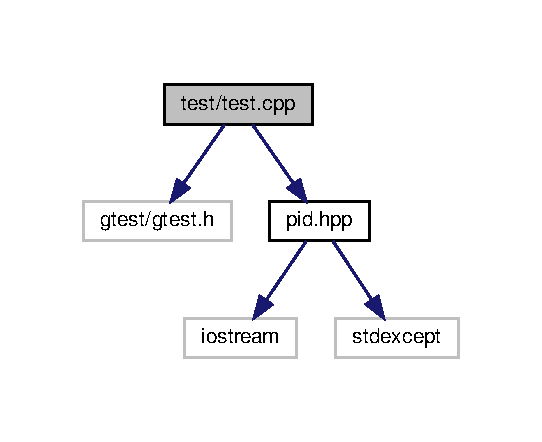
\includegraphics[width=260pt]{test_8cpp__incl}
\end{center}
\end{figure}
\subsection*{Functions}
\begin{DoxyCompactItemize}
\item 
\mbox{\Hypertarget{test_8cpp_a894885ab5c81a47317aae18112d7fdb3}\label{test_8cpp_a894885ab5c81a47317aae18112d7fdb3}} 
{\bfseries T\+E\+ST} (Invalid\+Dt, test\+\_\+check\+Parameters)
\item 
\mbox{\Hypertarget{test_8cpp_ae0321fa2770af09b769256a4d1e20c58}\label{test_8cpp_ae0321fa2770af09b769256a4d1e20c58}} 
{\bfseries T\+E\+ST} (Invalid\+Gains, test\+\_\+check\+Parameters)
\item 
\mbox{\Hypertarget{test_8cpp_a386448a90afc23bbac3130a6480c2818}\label{test_8cpp_a386448a90afc23bbac3130a6480c2818}} 
{\bfseries T\+E\+ST} (Valid\+Gains, test\+\_\+check\+Parameters)
\item 
\mbox{\Hypertarget{test_8cpp_a1580959438692082e280d4f3eb17ca27}\label{test_8cpp_a1580959438692082e280d4f3eb17ca27}} 
{\bfseries T\+E\+ST} (P\+I\+D\+Test, test\+\_\+compute\+Output)
\item 
\mbox{\Hypertarget{test_8cpp_a12490dde71fec2c28dbf8bfeb6c8546f}\label{test_8cpp_a12490dde71fec2c28dbf8bfeb6c8546f}} 
{\bfseries T\+E\+ST} (Saturation\+Test, test\+\_\+compute\+Output)
\item 
\mbox{\Hypertarget{test_8cpp_a007605857ec6c9af9bd9e42a37328c60}\label{test_8cpp_a007605857ec6c9af9bd9e42a37328c60}} 
{\bfseries T\+E\+ST} (Param\+Verification\+Test, verify\+Parameters)
\item 
\mbox{\Hypertarget{test_8cpp_a7bb9b552b62f768dbc753b9a99146b86}\label{test_8cpp_a7bb9b552b62f768dbc753b9a99146b86}} 
{\bfseries T\+E\+ST} (Integral\+Test, test\+\_\+integral)
\item 
\mbox{\Hypertarget{test_8cpp_a78a03229aaefe1a6a4c34c5b2cf8b77b}\label{test_8cpp_a78a03229aaefe1a6a4c34c5b2cf8b77b}} 
{\bfseries T\+E\+ST} (Derivative\+Test, test\+\_\+derivative)
\end{DoxyCompactItemize}


\subsection{Detailed Description}
Test file for \hyperlink{classPID}{P\+ID} Controller. 

\begin{DoxyAuthor}{Author}
Siddharth Telang (\href{mailto:stelang@umd.edu}{\tt stelang@umd.\+edu}) 

Dani Lerner (\href{mailto:dalerner@umd.edu}{\tt dalerner@umd.\+edu}) 
\end{DoxyAuthor}
\begin{DoxyVersion}{Version}
0.\+1 
\end{DoxyVersion}
\begin{DoxyDate}{Date}
2021-\/09-\/30
\end{DoxyDate}
Copyright (c) 2021 
%--- End generated contents ---

% Index
\backmatter
\newpage
\phantomsection
\clearemptydoublepage
\addcontentsline{toc}{chapter}{Index}
\printindex

\end{document}
